\section{Password Authentication}
\label{section:password-authentication}

Passwords are one of the most common and oldest forms of user authentication, being first used in computers at MIT in the mid-60s \cite{mcmillan2012password}.

We need to understand the high level model of password authentication, its risks and tools to mitigate it.

\subsubsection{Authentication Model}

% High level arch
Password based authentication is a simple model, based on a shared secret between the user and the system. The secret is referred to as a password, because the secret is usually a set of characters or words memorised by the user, inputted via a keyboard.
The password is often used in a combination with a username.

To authenticate the user exchanges the password with the system, and the system authenticates the user if the password is correct.

\begin{figure}[h]
	\centering
	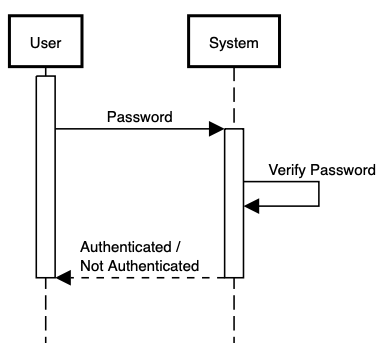
\includegraphics[height=8cm]{images/password-authentication}
	\caption{Password Authentication Model}
	\label{fig:password-authentication}
\end{figure}

\subsection{Security Vulnerabilities}
\label{label:password-vulnerabilities}

In a common password authentication system implementation used on the web, the user sends a plain-text password over a secure HTTPS connection, the server verifies it and responds.
The simplicity that makes passwords practical for users is what makes them a vulnerability for systems that rely on them.

Because passwords are supposed to be memorised and the proliferation of websites requiring them, users tend to pick password that are easier to remember and reuse passwords across different websites \cite{conklin2004password}.
Many websites also don't properly handle passwords, enabling attackers to access plain-text passwords when a security breach happens.
The industry is aiming to improve password security with the adoption of password managers and initiatives like FIDO \cite{cho2014passwordless} working to retire passwords altogether.

Attacks can be according to NIST \cite{grassi2017} classified as \textit{online} or \textit{offline}, based on wether the attacker is directly interacting with an authentication system.

%Security measures against online attacks can be implemented independently, regardless of the underlying authentication system, while offline attacks exploit data directly used by the authentication system.
%For this reason preventive measures need to be accounted for in the authentication system design.

\subsubsection{Online Attacks} An attack where an attacker is directly interacting with the authentication system.
These attacks are usually very \textit{noisy}, making it easy for an authentication system to detect it and react.
For example, locking an account after 5 failed authentication attempts.
For this reason, most online attacks are not very effective.

Effective online attacks work by operating under the radar of detection, for example, by trying out a small number of passwords on each user.
Popular methods are \textit{password spraying} and \textit{credential stuffing} \cite{haber2020attack}, both of which utilise information from data breaches, like lists of most commonly used passwords, or username and password combinations.
\textit{Password spraying} is taking a small number of commonly used passwords and attempting to authenticate with a large number of accounts, the attacker is assuming that in a large sample of accounts some will be using these weak passwords.
\textit{Credential stuffing} is taking a compromised user credential, for example a username and password combination found in a data breach, and using it to authenticate into multiple websites.
The attacker is assuming that if a person is using a set of credentials on one website, they are potentially reusing them on others.

\subsubsection{Offline Attacks}
Are attacks performed in a system controlled by the attacker.
For example, an attacker might analyse data on his personal computer to extract sensitive information.
The data is obtained by either theft of file, eavesdropping an authentication protocol or a system penetration.

\textit{Password cracking} \cite{blocki2018economics} is method of extracting user credentials from data used by the authentication system to verify users credentials.
The success of password cracking is generally determined by two parameters, the time required to check a single password and number of guesses required or the strength of the underlying password.

\subsubsection{Security Practices}
\label{password-security-practices}
There are many different things an authentication system can incorporate to improve its security.
An authentication system can adopt techniques for preventing active attacks and improving password strength independently of the underlying password verification methods.
We are going to be focusing on methods for handling passwords on the data layer, where we protect ourselves against offline attacks.
The form in which passwords exits on the data layer is also constrained by the ZKP protocol used for password verification.

\paragraph{Key-Stretching}
\label{paragraph:password-hashing}
Protecting passwords on the data layer is of critical importance.
\textit{Key-stretching} \cite{hornby2016salted} also called \textit{password hashing} is the industry standard method of improving security of low entropy secrets like passwords.

%An insecure system might store the passwords or password-equivalent data in plain text and compare them for verification. While simple, this system is insecure as user credentials directly are exposed with any unauthorised access.x
With this approach the password $p$ is \textit{stretched} or \textit{hashed} using a function $H$ and a high entropy value called a \textit{salt} $s$, the output called a \textit{password hash} $p_H$ and the salt are stored in persistent memory while the plain text password is discarded.
$$H(p, s) = p_H$$

When verifying the password $p'$, it is stretched again $H(p', s) = p{'}_H$ with the stored salt $s$ and the output hash $p{'}_H$ is compared with the stored password hash $p{'}_H \stackrel{?}{=} p_H$, if it matches the password is correct.

Key-stretching \cite{blocki2018economics} is traditionally done with hash iteration functions (PBKDF2, Bcrypt) \cite{kaliski2000pkcs, provos1999bcrypt}, these algorithms are CPU intensive, however are vulnerable to attackers with special purpose hardware (ASIC), so a better choice are memory-hard algorithms (Argon2, Scrypt, Balloon) \cite{biryukov2016argon2, percival2016scrypt, boneh2016balloon}.\\
%Because salt is stored alongside password hashes, systems sometimes also utilise a third value called \textit{pepper}, which is the same for all passwords, but stored in a different place from the salt.
%\newline
%When using a key stretching method with a function $H$, the password $p$ is stretched with a salt $s$, the password hash $p_H$ and salt $s$ are stored, while the password $p$ can be discarded.
%When authenticating the user, the system stretches the submitted password $p'$ with the stored salt $s$, and compares the hash $p{'}_H$ with the stored hash $p_H$ to know if the password is correct.
%
%

%\subparagraph{Password Strength}
%Measure of entropy with determines the difficulty of the password being guessed.
%Re-using passwords greatly undermines password strength and is what attacks like credential stuffing rely on.
%Have I Been Pwned \cite{hunt2021have} catalogs 613,584,248 passwords recovered from data breaches, while CrackStation \cite{hornby2019password} lists a collection of 1,493,677,782 words used for password cracking.
%Some papers \cite{blocki2018economics} have provided strong evidence that passwords follow a Zipf's law distribution.